%************************************************
\chapter{Einleitung}\label{ch:introduction}
%************************************************


%Here comes the introduction with a cite \cite{renz2016lak} and a ref \autoref{ch:conclusion} and an acronym \ac{API}.
%
%\begin{figure}[!h]
%	\centering
%	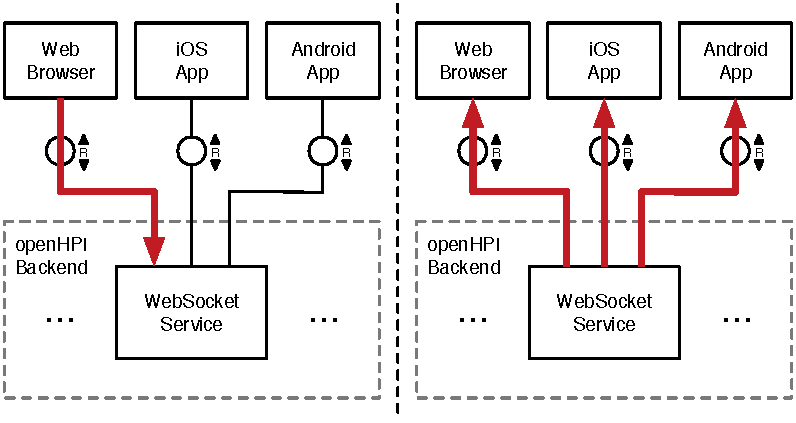
\includegraphics[width=0.8\textwidth]{figures/websocket}
%	\caption[A Figure Short-Title]{A Figure Title}
%	\label{fig:websocket}
%\end{figure}

\section{Motivation}
In den letzten Jahren hat sich das verwendete Datenvolumen des Internets immer weiter gesteigert. Laut Statista belief sich das weltweite Datenvolumen auf 33 Zettabyte und wird sich bis zum Jahr 2025 auf 175 Zettabyte steigern.\cite{statistica-datenvolumen} Zwar ist die vorhandene Bandbreite bei vielen Nutzern ebenfalls gestiegen, jedoch ist die Bandbreite, vor allem in ländlicheren Regionen oft noch nicht ausreichend.\cite{bmvi-bandbreite} Insbesondere wenn viele Nutzer sich gemeinsam eine Internet Anbindung teilen müssen ist dies ein Problem.

Immer mehr Unternehmen halten Ihre Hauptversammlungen, Kundgebungen, und Pressemitteilungen über Live Streams im Internet ab. Dies stellt sie vor das Problem das trotz oftmals guter Internetanbindung zu viele Mitarbeiter das Video über die Internetanbindung laden müssen, was zu einer vollständigen Auslastung des WANs führen kann. Dies wiederum kann zur Folge haben, dass ein Arbeiten für die restliche Belegschaft schwierig bis unmöglich wird. Der dadurch entstandene Schaden ist oft nur schwer zu beziffern, beläuft sich aber schon bei Mittelständischen Unternehmen auf bis zu 25000 Euro pro Stunde.\cite{zero-internet-schaden}

Nicht nur bei Unternehmen sondern auch in Schulen ist die Digitalisierung auf dem Vormarsch. Zunehmend werden Online-Lernplattformen im Unterricht eingesetzt. Diese Entwicklung wird jedoch stark ausgebremst durch fehlende Internet Bandbreiten. Viele Schulen haben eine schlechtere Internetanbindung als viele privat Haushalte.\cite{sonderstudie_digital} Um Inhalte anzeigen zu können, muss jeder Schüler einer Klasse sich diese über das WAN aus dem Internet herunterladen. Da jedoch Schüler in derselben Klasse oft die gleichen Inhalte benötigen, kann Bandbreite gespart werden, indem diese Inhalte nur einmal über das Internet geladen und anschließend im lokalen Netzwerk verteilt werden.

Beide Anwendungsfälle haben gemeinsam das viele Nutzer die selben Inhalte zur annähernd gleichen Zeit benötigen und zum aktuellen Zeitpunkt häufig über das Internet laden müssen. Diese Zeitliche und inhaltlich Lokalität kann genutzt werden um die benötigte Bandbreite zu reduzieren, indem die Inhalte nur einmal über das WAN geladen und anschließend im lokalen Netzwerk verteilt werden.

Die folgende Arbeit betrachtet den Anwendungsfall des Live-Streaming und den Einsatz von Unterstützender Software in Schulen. Es wird betrachtet ob ein Peer to Peer Ansatz zu einer Verbesserung von Ladezeiten und Netzwerklast betragen kann.
 


% https://de.statista.com/statistik/daten/studie/266869/umfrage/prognose-zum-datenvolumen-des-globalen-ip-traffics/

%\begin{table}[!h]
%\centering
%\begin{tabular}{@{}lllll@{}}
%\toprule
%Algorithm & Class & Precision & Recall & F-Measure \\ \midrule
%SVM       & CoP   & 0.309     & 0.486  & 0.378     \\ \cmidrule(l){2-5}
%          & RoA   & 0.571     & 0.560  & 0.565     \\ \midrule
%kNN       & CoP   & 0.391     & 0.344  & 0.366     \\ \cmidrule(l){2-5}
%          & RoA   & 0.623     & 0.660  & 0.641     \\ \midrule
%RForest   & CoP   & 0.493     & 0.262  & 0.342     \\ \cmidrule(l){2-5}
%          & RoA   & 0.639     & 0.851  & 0.730     \\ \bottomrule
%\end{tabular}
%\caption{My First Table}
%\label{tab:first-table}
%\end{table}

\section{Projekt \schulCloud}
%Das Projekt \schulCloud\footnote{https://schul-cloud.org/} ist eine webbasierte Lehr- und Lernplattform dessen Ziel es ist die Digitalisierung an Schulen zu fördern. Zusammen mit dem nationalen Excellence-Schulnetzwerk(MINTEC) wurde das Projekt vom \hpi 2016 ins leben gerufen. Im Mai 2017 startet die Pilotphase des Projektes mit insgesamt 27 Schulen. 
%Die Plattform soll Lehrer dabei unterstützen Unterrichtsstunden vorzubereiten, durchzuführen und Aufgaben an die Schüler zu verteilen. Auch die Verteilung von externen Materialien wie Bücher für die Schüler ist möglich.

Das Projekt \schulCloud\footnote{https://schul-cloud.org/} ist ein Gemeinschaftsprojekt des \hpi und des nationalen Execellence-Schulnetzwerkes (MINT-EC). Im Mai 2017 startete die Pilotphase des Projektes mit insgesamt 27 Schulen. Ziel des Projektes ist die Förderung der Digitalisierung in Schulen. 
Zu diesem Zweck wurde eine Web basierte Plattform entwickelt die Lehrer und Schüler bei der Unterrichtsvorbereitung, Durchführung und Nachbereitung unterstützen soll. 

Lehrer können Kurse anlegen und diese nutzen um Materialien sowie Aufgaben zu verteilen. Schülern ist es über die Plattform möglich Lösungen für Aufgaben einzureichen und ihr Ergebnis einzusehen. Über einen Kalender können sie Ihren Stundenplan abrufen.

Das Projekt wird als Open Source Projekt zur Verfügung gestellt und basiert auf einer Microservices Architektur. Bei diesem Architekturmuster wird die Software aus unabhängigen Softwarekomponenten(Services) zusammengesetzt. Die Komponenten kommunizieren über Schnittstellen, sind aber darüber hinaus eigenständige Entitäten und können von beliebig vielen anderen Komponenten verwendet werden. Durch die Verwendung von Microservices wird eine einfachere Anbindung an bestehende Infrastrukturen ermöglicht. Des weiteren können einzelne Services ersetzt werden um die Plattform an die Anforderungen der Schulen anzupassen. Bereitgestellt wird die Plattform mit Hilfe von Cloud Hosting, bei dem die Infrastruktur zentral und nicht von jeder Schule bereitgestellt wird. Dies ermöglicht eine einfache Skalierung. Neben der Web Anwendung existieren native Apps für Android und IOS.

%\note{unsicher wie detailliert ich hier werden soll}

%
%Gemeinschaftsprojekt
%	- HPI 2016
%	- MINT-EC
%	- BMF gefördert
%	- Förderung der Digitalisierung in Schulen
%	- Im Mai 2017 startet die Pilotphase des Projektes mit insgesamt 27 Schulen. 
%Bereitstellung von webbasierten Lerninhalten und Anwendungen über einen Zugang
%
%Kurse
%
%Kalender
%
%Dateien
%
%technischer Aufbau:

%Das Projekt wird als Open Source Projekt zur Verfügung gestellt und basiert auf Microservices. Der Plattform zu Grunde liegt ein Cloud Ansatz, bei dem die Infrastruktur zentral und nicht von jeder Schule bereitgestellt wird. Neben der Web Anwendung existieren native Apps für Android und IOS.


% kurse
% kalender
% dateien
%technischer aufbau

%Hasso-Plattner-Instituts (HPI) + nationalen Excellence-Schulnetzwerk (MINTEC).
%förderung der digitalisierung in schulen
%webbasierte anwendung
%Stundenvorbereitung
%hausaufgaben
%2016 ins leben gerufen
%micro services
%cloud architektur
%open source projekt
%native apps für android und ios
%bestehende anbieter nutzen/verbinden impl nur wenn noch nicht vorhanden
\section{Slidesync}
Slidesync\footnote{slidesync} ist eine Live Streaming Plattform des Unternehmens MediaEvent Services GmbH & Co. KG. Sie ermöglicht es Live-Streams eigenständig anzulegen und an eine Vielzahl von Nutzern zu verteilen. Die Zielgruppe der Plattform sind mittelständische bis große Unternehmen. Neben dem Self-Service, bei dem die Kunden selbst das Streaming übernehmen, wird auch ein Managed Service angeboten bei dem Media Event Services das Streaming und die Produktion vor Ort übernimmt. Die Plattform ist für eine große Anzahl von Nutzern ausgelegt und ist hochverfügbar um den Ansprüchen von Unternehmen gerecht zu werden. Sie stellt unter anderem Funktionen bereit um Events mit Registrierung und Foliensätzen zu realisieren. Die Plattform wird in Ruby on Rails entwickelt und stellt neben den Anwendungsservern auch eigene Streaming Server bereit.

\section{Ziele}
\subsection{Forschungsfrage}
\begin{itemize}
	\item Wie können in einem Netzwerk mit geringerer Internetanbindung Datenintensiven Ressourcen ausgeliefert werden?
	\item Eignet sich ein Peer to Peer Ansatz um die benötigte Internetbandbreite von Schulen und Unternehmen im Rahmen von Livestreams zu verbessern?
\end{itemize}
Diese Arbeit wird versuchen die Frage: 
Wie können in einem Netzwerk mit geringerer Internetanbindung Datenintensiven Ressourcen ausgeliefert werden? 
zu beantworten.

Dabei wird ein Fokus auf \pTp Technologien gesetzt. Zur Evaluation wird neben simulierten Benchmarks auch der Einsatz unter realen Bedingung getestet.  

%
%
%Um statische Inhalte anzeigen zu können, muss jeder Schüler einer Klasse sich diese aus dem Internet über ein Content Delivery Network(CDN) herunterladen. Da jedoch Schüler in derselben Klasse oft die gleichen Inhalte benötigen, kann Bandbreite gespart werden, indem diese Inhalte nur einmal über das Internet geladen und anschließend im lokalen Netzwerk verteilt werden. Um die benötigte Bandbreite zu reduzieren, wird untersucht ob sich ein Peer to Peer Ansatz zur Verteilung statischer Inhalte eingesetzt werden kann.
%
%Mit Hilfe von Webrtc werden die Inhalte direkt zwischen den Browsern ausgetauscht, ohne das ein externer Server benötigt wird. WebRTC ist ein offener Standard und ermöglicht es Browser paarweise zwecks Datenaustausch zu verbinden. Der große Vorteil dieser Technologie ist, dass sie direkt von modernen Browsern unterstützt wird, wodurch keine zusätzliche Software installiert werden muss. Für die Implementation wird für das Zwischenspeichern von Daten ein Serviceworker eingesetzt. Serviceworker können wie ein Proxy zwischen dem Webbrowser und dem Webserver agieren, welcher die Webseite bereitstellt. Stellt ein Browser eine Anfrage, so wird diese vom Serviceworker abgefangen. Der Serviceworker schaut zunächst in seinem Cache, der sog. IndexDB, ob er die gestellte Anfrage beantworten kann. Ist dies nicht der Fall, so wird die Anfrage an den Webserver weitergeleitet. Wird die gleiche Anfrage nochmals gestellt, kann diese aus dem Cache beantwortet werden, da gestellte Anfragen eine gewisse Zeit lang zwischengespeichert werden. Wird nun eine Ressource benötigt kann diese bei einem anderen Client, der sie zwischengespeichert hat, angefordert werden. Ist die Verbindung zwischen den Clients aufgebaut, ist ein Austausch von Daten auch dann noch möglich, wenn die Internetverbindung ausfällt.
%
%Im Rahmen eines Projekt Seminars konnte gezeigt werden, dass es technisch möglich ist auch große Inhalte über einen Peer to Peer Ansatz an Nutzer zu verteilen. Neben der Praxistauglichkeit werden nun in einer Masterarbeit die folgenden Themen genauer untersucht:
%\\
%\\
%\textbf{Serialisierung der Daten:}
%\\Für den Austausch von Daten werden die von WebRTC angebotene DataChannel genutzt, welche das Stream Control Transmission Protocol kurz SCTP verwendet. Problem hierbei ist, dass dieses Protokoll ursprünglich für die Übertragung von Kontrollinformationen designt wurde und deshalb für die Kompatibilität verschiedener Browser eine Paketgröße von 16kiB nicht überschritten werden sollte. In unserem Kontext ist es aber notwendig auch größere Dateien zu übertragen, weshalb aktuell viele kleine Datenpakete verwendet werden müssen. Hierdurch entsteht ein nicht zu vernachlässigender Overhead.
%\\
%\\
%\textbf{Integrität der Daten:}
%\\Es muss verhindert werden, dass ein bösartiger Nutzer manipulierte Ressourcen im lokalen Netzwerk verbreiten kann. Hierzu kann die Integritätsüberprüfung von HTML5 verwendet werden, bei der die Integrität der Daten mittels einer Prüfsumme sichergestellt wird.
%\\
%\\
%\textbf{Verteilung der Daten in größeren Gruppen:}
%\\Für den Austausch von Daten bilden aktuell alle Teilnehmer ein vollständig vermaschtes Netz. Bei einer Klassengröße von 30 hat also jeder Browser 29 offene DataChannels. Denkt man beispielsweise an eine Vollversammlung mit etwa 1000 Schülern, kann die große Anzahl der offenen DataChannels zu Problemen führen. In solche Szenarien sollt eine andere Topologie eingesetzt werden um die Anzahl der offenen DataChannels zu reduzieren. Am sinnvollsten wäre hier eine baumartige oder irregulär vermaschte Topologie.
%\\
%\\
%\textbf{Evaluierung der Performance:}
%\\Ziel der Softwarelösung ist es, die Benutzbarkeit von Internetseiten in Anwesenheit einer schlechten Internetanbindung zu verbessern. Interessant wäre es, den Performancezuwachs zu evaluieren, der durch den Einsatz unserer Lösung erzeugt wird. So könnte auch evaluiert werden, bis zu welcher zur Verfügung stehenden Datenrate der Einsatz unserer Lösung sinnvoll ist.
%\\
%\\
%\textbf{Verwaltung des Caches:}
%\\Wie bereits beschrieben, wird für die Zwischenspeicherung der Daten einen Serviceworker eingesetzt, welcher wiederum die IndexDB verwaltet. Für die Zukunft sollte eine Lösung dafür gefunden werden ein sinnvolles Zeitfenster festzulegen in dem die Zwischengespeicherten Daten gültig sind, damit keine veralteten Daten ausgetauscht werden. Ein weiterer Punkt ist die Größe des Caches. Hier sollte evaluiert werden, wie die Maximalgröße des Caches und dessen Performance dabei ist. In Anlehnung hieran sollte eine Obergrenze für die menge der zwischengespeicherten Daten festgelegt werden.
%
